
\de{ĐỀ THI HỌC KỲ I NĂM HỌC 2022-2023}{THPT Lê Quý Đôn}


\begin{bt}%[Đề kiểm tra HK1 môn Toán 10 trường THPT Lê Quý Đôn]%[Đoàn Minh Tân, 10EX-HK1-2223]%	[0D4B4-2]
	Biểu diễn miền nghiệm của hệ bất phương trình $\heva{& 2x+3y\le 12\\ & x\ge 0\\ &y\ge 0.}$
	\loigiai{
		Vẽ đường thẳng $d\colon 2x+3y=12$ đi qua hai điểm $A(6,0)$ và $B(0,4)$.
		\begin{center}
			\begin{tikzpicture}[line cap=round, line join=round, font=\footnotesize, >=stealth, scale=0.6]
				\tikzset{label style/.style={font=\footnotesize}}
				%---------- vẽ hệ trục tọa độ
				\draw[->] (-2,0)--(8,0) node[below right] {$x$};
				\draw[->] (0,-2)--(0,5) node[right] {$y$};
				\node (0,0) [above right] {$ O $};
				%---------- đoạn chắn trên trục
				\foreach \x in {-1,1,2,3,4,5,6,7}
				\draw[shift={(\x,0)},color=black] (0pt,2pt) -- (0pt,-2pt);
				\foreach \y in {-1,1,2,3,4}
				\draw[shift={(0,\y)},color=black] (2pt,0pt) -- (-2pt,0pt);
				
				%---------- vẽ hàm
				\draw [domain=-1.5:8, samples=100] plot (\x, {(12-2*(\x))/3});
				\node at (2.2,2) {$d$};
				
				%---------- vẽ miền nghiệm
				\draw[pattern=north east lines, draw=none] (-1.5,5) -- (8,5) -- (8,-1.33)--cycle;
				\draw[pattern= north west lines, draw=none] (-2,5) -- (0,5) -- (0,-2)--(-2,-2)--cycle;
				\draw[pattern= vertical lines, draw=none] (-2,0) -- (8,0) -- (8,-2)--(-2,-2)--cycle;
				\draw[fill=black] (6,0) circle(1pt) node[below]{$A$} (0,4) circle(1pt) node[left]{$B$};
			\end{tikzpicture}
		\end{center}
		Vậy miền nghiệm của hệ bất phương trình đã cho là miền tam giác $OAB$ như hình vẽ.
	}
\end{bt}
\begin{bt}%[Đề kiểm tra HK1 môn Toán 10 trường THPT Lê Quý Đôn]%[Đoàn Minh Tân, 10EX-HK1-2223]%	[0D2B1-2]
	Tìm tập xác định $\mathscr{D}$ của hàm số $f(x)=\sqrt{4-x}+\dfrac{1}{x}$.
	\loigiai{
		Hàm số xác định khi và chỉ khi $\heva{& 4-x\ge 0\\ & x\ne 0}\Leftrightarrow \heva{& x\le 4\\ & x\ne 0.}$\\
		Vậy tập xác định của hàm số là $\mathscr{D}=(-\infty;4]\setminus \{0\}$.
	}
\end{bt}
\begin{bt}%[Đề kiểm tra HK1 môn Toán 10 trường THPT Lê Quý Đôn]%[Đoàn Minh Tân, 10EX-HK1-2223]%	[0D2K1-3]
	Xét sự biến thiên của hàm số $y=x^2-4x+5$ trên $(-\infty;2)$.
	\loigiai{
		Đặt $y=f(x)=x^2-4x+5$.\\
		Xét $x_1$, $x_2 \in (-\infty;2)$ sao cho $x_1<x_2$. Ta có
		\begin{eqnarray*}
			f\left(x_1\right)-f\left(x_2\right)&=&x_1^2-4x_1+5-\left(x_2^2-4x_2+5\right)\\
			&=&\left(x_1^2-x_2^2\right)-4\left(x_1-x_2\right)\\
			&=&\left(x_1-x_2\right)\left(x_1+x_2\right)-4(x_1-x_2)\\
			&=&\left(x_1-x_2\right)\left(x_1+x_2-4\right).
		\end{eqnarray*}
		Do $x_1<x_2$ nên $x_1-x_2<0$.\\
		Lại có $x_1$, $x_2 \in (-\infty;2)$ nên $x_1<2$, $x_2<2$, suy ra $x_1+x_2<4$ hay $x_1+x_2-4<0$.\\
		Do đó $f\left(x_1\right)-f\left(x_2\right)=\left(x_1-x_2\right)\left(x_1+x_2-4\right)>0.$\\
		Vậy hàm số $y=x^2-4x+5$ nghịch biến  trên $(-\infty;0)$.
	}
\end{bt}
\begin{bt}%[Đề kiểm tra HK1 môn Toán 10 trường THPT Lê Quý Đôn]%[Đoàn Minh Tân, 10EX-HK1-2223]%[0D2B3-2]
	Cho hàm số $y=ax^2+bx+3$ có đồ thị $(P)$. Tìm $a$, $b$ biết $(P)$ có đỉnh $I(2;-1)$.
	\loigiai{
		Parabol $(P)$ có đỉnh $I(2;-1)$ nên ta có hệ $\heva{& 4a+2b+3=-1\\ & -\dfrac{b}{2a}=2}\Leftrightarrow \heva{& 4a+2b=-4\\ & 4a+b=0}\Leftrightarrow \heva{& a=1\\ &b=-4.}$
		Vậy $(P)\colon y=x^2-4x+3$.
	}
\end{bt}

\begin{bt}%[Đề kiểm tra HK1 môn Toán 10 trường THPT Lê Quý Đôn]%[Đoàn Minh Tân, 10EX-HK1-2223]%	[0D2T3-5]
	\immini{Tại một khu hội chợ, người ta thiết kế cổng chào có hình parabol hướng bề lõm xuống dưới. giả sử lập một hệ trục toạ độ $Oxy$ sao cho một chân cổng đi qua gốc toạ độ $O$ như hình vẽ ($x$ và $y$ tính bằng mét). Chân kia của cổng ở vị trí $(4;0)$. Biết một điểm $M$ trên cổng có toạ độ $(1;3)$. Hỏi chiều cao của cổng (vị trí cao nhất của cổng tới mặt đất) là bao nhiêu mét?
	}
	{
		\begin{tikzpicture}[scale=0.7, font=\footnotesize, line join=round, line cap=round, >=stealth]
			\draw[->] (-1,0)--(5,0) node[below] {$x$};
			\draw[->] (0,-1)--(0,5) node[left] {$y$};
			\draw (0,0) node [below right] {$O$};
			\draw[samples=200,domain=0:4,smooth,variable=\x] plot (\x,{-(\x)^2+4*(\x)});
			\draw[dashed] (1,0)|-(0,3);
			\draw[fill=black] (1,0) circle(1pt) node[below]{$1$} (4,0) circle(1pt) node[below]{$4$} (0,3) circle(1pt) node[left]{$3$} (1,3) circle(1pt) node[right]{$M$} (0,0) circle(1pt);
		\end{tikzpicture}
	}
	\loigiai{
		Giả sử parabol $(P)$ có dạng $y=ax^2+bx+c$, $a\ne 0$.\\
		Dựa vào đồ thị, $(P)$ đi qua ba điểm $O(0,0)$, $M(1,3)$ và $A(4,0)$ nên ta có hệ phương trình $$\heva{& c=0\\ & a+b+c=3\\ & 16a+4b+c=0}\Leftrightarrow \heva{& c=0\\ & a+b=3\\ & 16a+4b=0}\Leftrightarrow \heva{& a=-1\\ & b=4\\ & c=0.}$$
		Suy ra $(P)\colon y=-x^2+4x$.\\
		Suy ra $(P)$ có đỉnh $I(2;4)$.\\
		Vậy chiều cao của cổng là $4$ mét.	
	}
\end{bt}



%==Bài 6==
\begin{bt}%[0T5B2-2][Dự án đề kiểm tra HKII NH22-23- Nguyễn Cường]%[THPT Lê Quý Đôn]
	Cho hình bình hành $ ABCD $ và điểm $ M $ tùy ý. Chứng minh 
	$ \overrightarrow{MA} +\overrightarrow{MC}=\overrightarrow{MB}+\overrightarrow{MD} $.
	\loigiai{
		\immini{
		Do $ABCD$ là hình bình hành nên $\overrightarrow{BC}=\overrightarrow{AD}$.\\
		Suy ra $\overrightarrow{BC}+\overrightarrow{DA}=\overrightarrow{0}$.\\
		Ta có 
		\allowdisplaybreaks
		\begin{eqnarray*}
			\overrightarrow{MA} +\overrightarrow{MC}&=&\overrightarrow{MB}+\overrightarrow{BC}+\overrightarrow{MD}+\overrightarrow{DA}\\
			&=&\overrightarrow{MB}+\overrightarrow{MD}+\overrightarrow{BC}+\overrightarrow{DA}\\
			&=&\overrightarrow{MB}+\overrightarrow{MD}.
		\end{eqnarray*}
	}
{
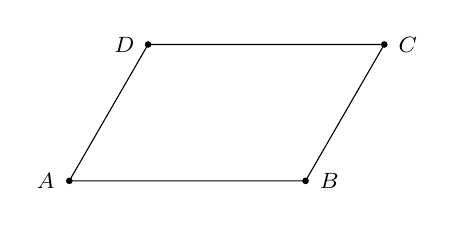
\begin{tikzpicture}[>=stealth,line join=round,line cap=round,font=\footnotesize,scale=1]
	\path (0,0) coordinate (A)++(0:3)coordinate(B)++(60:2)coordinate(C)++(180:3)coordinate(D);
	\draw (A)--(B)--(C)--(D)--cycle;
 \foreach \p / \r in {A/180,C/0,B/0,D/180}
	\fill (\p) circle (1.2pt) node[shift={(\r:3mm)}]{$\p$};
\end{tikzpicture}
}
}
\end{bt}
%==Bài 7==
\begin{bt}%[0T5K4-6][Dự án đề kiểm tra HKII NH22-23- Nguyễn Cường]%[THPT Lê Quý Đôn]
	Cho hình thang vuông $ ABCD $ có hai đáy $ AB=a $, $ CD=b $ và chiều cao $ AD=h $. Gọi $ M $ là trung điểm cạnh $ BC $. Biết rằng $ h^2=a^2+ab $. Tính góc giữa $ AM $ và $ BD $.
	\dapso{ $ 90^\circ $}
	\loigiai{\begin{center}
			\begin{tikzpicture}[>=stealth,line join=round,line cap=round,font=\footnotesize,scale=1]
				\path (0,0) coordinate (D)
				(D)++(90:2) coordinate (A)++(0:3)coordinate(B)
				(D)++(0:4) coordinate (C)
				($(B)!.5!(C)$)coordinate(M)
				;
				\draw (B)--(A)node[midway,above]{$a$};
				\draw (A)--(D)node[midway,left]{$h$};
				\draw (D)--(C)node[midway,below]{$b$};
				\draw (D)--(B)--(C) (A)--(M);
				\foreach \p / \r in {A/90,C/0,B/90,D/-90,M/45}
				\fill (\p) circle (1.2pt) node[shift={(\r:3mm)}]{$\p$};
			\end{tikzpicture}
		\end{center}
	Do $M$ là trung điểm $BC$ nên $\overrightarrow{AC}+\overrightarrow{AB}=2\overrightarrow{AM}$.\\
	Khi đó
	\allowdisplaybreaks
	\begin{eqnarray*}
		&&2\overrightarrow{AM}\cdot \overrightarrow{BD}\\
		&=&\left(\overrightarrow{AC}+\overrightarrow{AB}\right)\cdot\left(\overrightarrow{BA}+\overrightarrow{AD}\right)\\
		&=&\left(\overrightarrow{AD}+\overrightarrow{DC}+\overrightarrow{AB}\right)\cdot\left(\overrightarrow{BA}+\overrightarrow{AD}\right)\\
		&=&\overrightarrow{AD}\cdot\overrightarrow{BA}+\overrightarrow{AD}\cdot\overrightarrow{AD}+\overrightarrow{DC}\cdot\overrightarrow{BA}+\overrightarrow{DC}\cdot\overrightarrow{AD}+\overrightarrow{AB}\cdot\overrightarrow{BA}+\overrightarrow{AB}\cdot\overrightarrow{AD}\\
		&=&h^2-ab-a^2\\
		&=&a^2+ab-ab-a^2=0.
	\end{eqnarray*}
Do đó, $AM\perp BD$ hay góc giữa $AM$ và $BD$ là $90^\circ$.
	}
\end{bt}
%==Bài 8==
\begin{bt}%[0T5K2-5][Dự án đề kiểm tra HKII NH22-23- Nguyễn Cường]%[THPT Lê Quý Đôn]
	Cho ba lực $ F_1= \overrightarrow{MA}$, $ F_2= \overrightarrow{MB}$, $ F_3= \overrightarrow{MC}$ cùng tác động vào một vật tại điểm $ M $ và vật đứng yên. Cho biết cường độ của $ F_1 $, $ F_2 $ đều bằng $ 50N $ và góc $ \widehat{AMB}=60^\circ $. Tính cường độ của lực $ F_3 $.
	\dapso{$ 50\sqrt{3} $ }
	\loigiai{
		\immini{
				Vì vật đứng yên nên ta có
				\[\begin{aligned}
					\overrightarrow{F_1} + \overrightarrow{F_2} + \overrightarrow{F_3} = \overrightarrow{0} &\Rightarrow \overrightarrow{F_1} + \overrightarrow{F_2} = -\overrightarrow{F_3} \\
					&\Rightarrow \left( \overrightarrow{F_1} + \overrightarrow{F_2}\right)^2 = \left(-\overrightarrow{F_3}\right)^2  \\
					&\Rightarrow MA^2 + 2\overrightarrow{MA}\cdot\overrightarrow{MB} + MB^2 = MC^2 \\
					&\Rightarrow 50^2 + 2\cdot50\cdot50\cdot\cos60^\circ + 50^2 = MC^2\\
					&\Rightarrow MC = 50\sqrt{3}.
				\end{aligned}\]
				Vậy cường độ của lực $\overrightarrow{F_3}$ là $50\sqrt{3}$ N.
			}
		{
		\begin{tikzpicture}[>=stealth,line join=round,line cap=round,font=\footnotesize,scale=0.7]
			\path (0,0) coordinate (M)
			(M)++(30:2) coordinate (A)
			(M)++(-30:2) coordinate (B)
			($(A)+(B)-(M)$)coordinate (D)
			($(M)!-1!(D)$)coordinate (C)
			;
			\draw[->] (M)--(A)node[midway,above]{$\overrightarrow{F}_1$};
			\draw[->] (M)--(B)node[midway,below]{$\overrightarrow{F}_2$};
			\draw[->] (M)--(C)node[midway,above]{$\overrightarrow{F}_3$};
			\draw[->] (M)--(D);
			\draw[dashed] (B)--(D)--(A);
			\foreach \p / \r in {A/90,C/180,B/-90,M/90,D/0}
			\fill (\p) circle (1.2pt) node[shift={(\r:3mm)}]{$\p$};
		\end{tikzpicture}
	}
}
\end{bt}
%==Bài 9==
\begin{bt}%[0T6B2-1][Dự án đề kiểm tra HKII NH22-23- Nguyễn Cường]%[THPT Lê Quý Đôn]
Theo dõi số vụ va chạm giao thông mỗi ngày tại một giao lộ, kết quả được ghi lại ở bảng sau
\begin{center}
	\begin{tabular}{|c|c|c|c|c|c|c|}
		\hline
		Số vụ va chạm  &$0 $ &$1$ &$ 2 $ &$3 $ &$4 $ &$ 5 $\\
		\hline
		Số ngày & $4$ & $ 9 $& $ 2 $ & $ 7$ & $ 3 $ &$ 1 $ \\
		\hline
	\end{tabular}
\end{center}
Tính số trung bình, tứ phân vị và mốt của bảng kết quả trên.\\
	\dapso{  $\overline{x}=1{,}96$; $ Q_1=1 $; $ Q_2=1{,}5 $; $ Q_3=3 $; $ M_0=1 $}
	\loigiai{
		Số trung bình là $\overline{x}=\dfrac{4\cdot 0+9\cdot 1+2\cdot 2+7\cdot 3+3\cdot 4+1\cdot 5}{4+9+2+7+3+1}=1{,}96$.\\
		Cỡ mẫu là $n=26$ khi xếp số vị va chạm theo thứ tự không giảm thì số liệu thứ $13$ và $14$ là $1$ và $2$ nên tứ phân vị thứ hai là $Q_2=\dfrac{1+2}{2}=1{,}5$.\\
		Tứ phân vị thứ nhất là trung vị của $0$; $0$; $0$; $0$;$1$; $1$; $1$; $1$; $1$; $1$; $1$; $1$; $1$ là $Q_1=1$.\\
		Tứ phân vị thứ ba là trung vị của $2$; $2$; $3$; $3$;$3$; $3$; $3$; $3$; $3$; $4$; $4$; $4$; $5$ là $Q_3=3$.\\
		Mốt của bảng kết quả là $M_0=1$.
	}
\end{bt}
